\documentclass[11pt]{article}

\usepackage{sectsty}
\usepackage{graphicx}
\usepackage{enumitem}
\usepackage{listings}
\usepackage{xcolor}
\usepackage{graphicx}
\usepackage{fancyhdr}
\usepackage{epigraph} 

\definecolor{codegreen}{rgb}{0,0.6,0}
\definecolor{codegray}{rgb}{0.5,0.5,0.5}
\definecolor{codepurple}{rgb}{0.58,0,0.82}
\definecolor{backcolour}{rgb}{0.95,0.95,0.92}

\lstdefinestyle{mystyle}{
    backgroundcolor=\color{backcolour},   
    commentstyle=\color{codegreen},
    keywordstyle=\color{magenta},
    numberstyle=\tiny\color{codegray},
    stringstyle=\color{codepurple},
    basicstyle=\ttfamily\footnotesize,
    breakatwhitespace=false,         
    breaklines=true,                 
    captionpos=b,                    
    keepspaces=true,                 
    numbers=left,                    
    numbersep=5pt,                  
    showspaces=false,                
    showstringspaces=false,
    showtabs=false,                  
    tabsize=2
}

\lstset{style=mystyle}


% Margins
\topmargin=-0.45in
\evensidemargin=0in
\oddsidemargin=0in
\textwidth=6.5in
\textheight=9.0in
\headsep=0.25in

\title{ Web Technology Solution\\2020 Spring}

\author{ Sanjaya (Bir Bikram) Shrestha }
\date{\today}



\begin{document}
\maketitle	
\pagestyle{fancy}
\fancyhead[RO,LE]{\textbf{WT Solution 2020 Spring}}
\fancyfoot[RO,RE]{By: Sanjaya (Bir Bikram) Shrestha}

\tableofcontents
\pagebreak

% Optional TOC
% \tableofcontents
% \pagebreak

%--Paper--

\section{(Q No.1 A) What happens if you enter https://pu.edu.np into your browsers? Describe the procedures behind the scenes. Describe along with its block diagram.}
\subparagraph{}
When we type the https://pu.edu.np following sequence of events will happen behind the scene.

\begin{enumerate}
    \item Browser will initiates a request to the Domain Name System (DNS) to resolve the domain name "pu.edu.np" into an IP address.
    \item The DNS responds with the IP address associated with the domain name, which in this case is the IP address of the server hosting the website.
    \item Browser will initiates a secure connection with the server using HTTPS protocol, which includes a series of handshaking and authentication steps to ensure the connection is secure and encrypted.
    \item The server responds with the HTML code for the home page of the pu.edu.np website.
    \item Browser then receives the HTML code and begins to parse it to render the page.
    \item The browser sends additional requests for any external files referenced in the HTML code, such as CSS stylesheets, images, and scripts.
    \item The server responds with the requested files and the browser uses them to render the page as intended.
    \item Then if we interact with the website, such as clicking a link or submitting a form, the browser sends additional requests to the server and the server responds with the appropriate content.
\end{enumerate}

\begin{lstlisting}
                            +---------------------+
                            | DNS Resolution      |
                            +---------------------+
                                        |
                                        v
    +------------+          +-----------------------+
    | Browser    |          | HTTPS Handshaking      |
    +------------+          +-----------------------+
            |                        |
            v                        v
    +-------------------+  +---------------------------+
    | Receive HTML code |  | Receive external resources |
    +-------------------+  +---------------------------+
            |                        |
            v                        v
    +-------------------+  +------------------------+
    | Parse HTML code   |  | Render page with assets |
    +-------------------+  +------------------------+
            |                        |
            v                        v
    +------------------+  +------------------+
    | Interact with website          |
    +------------------+  +------------------+

\end{lstlisting}

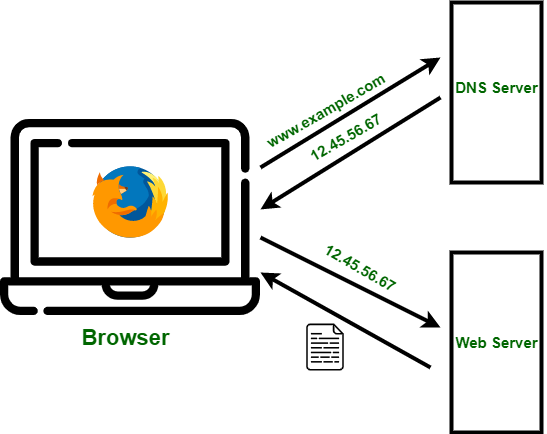
\includegraphics[width=0.5\textwidth]{resources/qno1a.png}


\noindent\rule{\linewidth}{0.4pt}
\section{(Q No.2 Differentiate between inline, internal and external CSS with an example? Int he code snippet below, what would be the color of both elements 1 and 2? Also explain why?) }
\begin{lstlisting}[language=html]
    style.min.css
    #about p.element-2{color:red;}
    .about p.element-2{color:black;}

    index.html

    ----------
    <div id="about" class="about">
        <p class="element-2"> <!-- Element 1 -->
            All right reserved
        </p>
        <p id="element-2"> <!-- Element 2 -->
            I love Web Technology
        </p>

    </div>
\end{lstlisting}
\subparagraph{}

CSS (Cascading Style Sheets) is a styling language used to apply styles to HTML elements. There are three ways to add CSS to an HTML document: inline, internal, and external.

\begin{itemize}
    \item \textbf{Inline CSS:} Inline CSS is when you apply styles directly to an HTML element using the "style" attribute. Here's an example:
    \begin{lstlisting}[language=html]
        <h1 style="color: blue;">This is an inline heading</h1>
    \end{lstlisting}
    
    In this example, the "style" attribute is used to set the color of the h1 element to blue. Inline CSS is typically used for quick styling fixes or for styles that only apply to a single element.
    
    \item \textbf{Internal CSS:} Internal CSS is when you define styles within the $<$head$>$ section of an HTML document, using the $<$style$>$ tag. Here's an example:
    \begin{lstlisting}[language=html]
        <head>
        <style>
            h1 {
            color: blue;
            }
        </style>
        </head>
        <body>
        <h1>This is an internal heading</h1>
        </body>
    \end{lstlisting}
    In this example, the "style" element is used to define a style for the h1 element. Internal CSS is typically used for styling multiple elements on a single page.
    
    \item \textbf{External CSS:} External CSS is when you define styles in a separate file and link to it in the $<$head$>$ section of an HTML document. Here's an example:
    
    \begin{lstlisting}[language=html]
        <head>
        <link rel="stylesheet" type="text/css" href="styles.css">
        </head>
        <body>
        <h1>This is an external heading</h1>
        </body>
     
    \end{lstlisting}
    In this example, the "link" element is used to link to an external CSS file called "styles.css", which contains the styles for the h1 element. External CSS is typically used for styling multiple pages across a website.
    
\end{itemize}

In the given code, \\the color of element 1 will be red and\\ the color of element 2 will be black.

This is because of the CSS selector specificity. The selector \#about p.element-2 has a higher specificity than .about p.element-2, because it includes an ID selector \#about which has a higher specificity than a class selector .about. So, for the element with class element-2 inside the \#about div, the first selector will be applied, which sets the color to red.

On the other hand, the element 2 has a id of element-2 but it doesn't have an class of element-2, so css is specified to work for p element with id element-2 so the default style will be applied so the color will be set to black.


\noindent\rule{\linewidth}{0.4pt}
\section{(Q No.3 Write a program to display the following output.) }
% todo: load image

\lstinputlisting[language=html, caption={Table in Html}]{resources/qno3.html}





\noindent\rule{\linewidth}{0.4pt}
\section{(Q No.4 "JavaScript programs the behaviour of the webpage". Explain this statement with suitabel example. Employ DOM event model in JavaScript to illustrate the dragging and dropping of element with suitabel example.) }
\subparagraph{}
The statement "JavaScript programs the behavior of the webpage" means that JavaScript is used to add interactivity and dynamic functionality to a webpage. Here's an example to explain this:

Suppose we have a webpage with a button that when clicked, displays a message. We can achieve this using JavaScript.

First, we need to add an event listener to the button so that it listens for when the button is clicked. We can do this using the addEventListener() method in JavaScript:

\begin{lstlisting}[language=html]
    <button id="myButton">Click me</button>

    <script>
    const button = document.getElementById("myButton");

    button.addEventListener("click", function() {
        alert("Hello, world!");
    });
</script>

\end{lstlisting}

\lstinputlisting[language=html, caption={Drag and Drop}]{resources/qno4.html}
To make an element draggable we set the draggable attribute to true of the element.
The ondragstart attribute calls a function, drag(event), that specifies what data to be dragged.

The dataTransfer.setData() method sets the data type and the value of the dragged data:
The ondragover event specifies where the dragged data can be dropped.


\noindent\rule{\linewidth}{0.4pt}
\section{(Q No.5A What are the different types of Array in PHP? Explain the details with syntax(Use the name of your friend as example)) }
\subparagraph{}
In PHP, there are three types of arrays:
\begin{enumerate}
    \item \textbf{Indexed arrays:}
    An indexed array stores a collection of values, each of which is assigned a numeric index. The index starts at 0 and increases by 1 for each element in the array. Indexed arrays can be created using the array() function or using the shorthand [] syntax. Here's an example:
    \begin{lstlisting}[language=php]
        $names = array("ram", "shyam", "hari");
        // or
        $names = ["ram", "shyam", "hari"];
    \end{lstlisting}

    \item \textbf{Associative arrays:}
    An associative array stores a collection of key-value pairs, where each key is a string and each value can be of any type. Associative arrays can be created using the \[array()\] function or using the shorthand [] syntax, but the key-value pairs must be explicitly defined using the =$>$ operator. Here's an example:
    \begin{lstlisting}[language=php]
        $person = array("name" => "John", "age" => 30, "email" => "john@example.com");
        // or
        $person = ["name" => "John", "age" => 30, "email" => "john@example.com"];

    \end{lstlisting}

    \item \textbf{Multi dimensional array:}
    Multidimensional array is an array that contains one or more arrays as its elements. Each element of a multidimensional array can be an array itself, which can contain further arrays as its elements.

    Multidimensional arrays are useful for representing complex data structures, such as tables or matrices. They can be indexed using multiple sets of keys, which allows for flexible and efficient data access.
    \begin{lstlisting}[language=php]
        $data = array(
            array("John", "Doe", 25),
            array("Jane", "Smith", 30),
            array("Bob", "Johnson", 40)
        );
    \end{lstlisting}
\end{enumerate}


\noindent\rule{\linewidth}{0.4pt}
\section{(Q No.5B What role do cookies and session play in allowing web servers to store stateful data? Give example to illustrate your point.}
\subparagraph{}
Cookies and sessions are both used to allow web servers to store stateful data, which means data that persists across multiple requests.

Cookies are small text files that are stored on the client-side (i.e. on the user's browser). They are typically used to store user preferences, login information, shopping cart items, and other small amounts of data that need to persist between visits to a website. Cookies are sent to the server with every request, so the server can read and modify the contents of cookies to store and retrieve stateful data.

Sessions, on the other hand, are stored on the server-side. When a user visits a website, the server creates a session for that user and assigns a unique identifier (usually a session ID) to that session. The session ID is then sent to the client in the form of a cookie, so that the server can identify the user in subsequent requests. The server can then store stateful data related to that user in the session, and retrieve it as needed.
\\
Here's an example to illustrate how cookies and sessions can be used to store stateful data:

Suppose we have an online store where users can add items to their shopping cart. When a user adds an item to their cart, we want to store that information so that it persists even if the user navigates away from the site and comes back later.

We can use cookies to store the shopping cart items on the client-side. Each time the user adds an item to their cart, we can update a cookie with the item details. Then, when the user returns to the site, we can read the contents of the cookie and display the items in their cart.

However, cookies have limitations in terms of storage capacity and security. To store sensitive data like payment information, we need a more secure and reliable way to store stateful data. That's where sessions come in. We can create a session for each user and store their shopping cart items in the session. This way, the data is stored on the server-side and is more secure than using cookies. We can also store larger amounts of data in a session than we can in a cookie.

In summary, cookies and sessions are both used to store stateful data, but they have different properties and use cases. Cookies are typically used for small amounts of data that need to persist on the client-side, while sessions are used for larger amounts of data and more sensitive data that needs to be stored on the server-side.

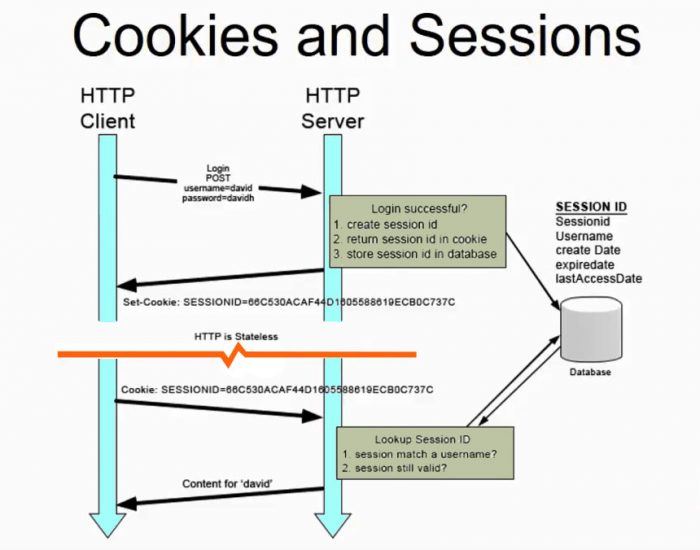
\includegraphics[width=0.75\textwidth]{resources/session_cookie.jpg}


\noindent\rule{\linewidth}{0.4pt}
\section{(Q No.6 Prepare a login form with input field username/email and password and also the option for remembering the login session. Write PHP MySQL code to establish the database connection and verify the user and successfully login and establish login session for valid users and show error messages if invalid. Use the client and server side validation, along with pattern matching implemented to allow only authorized user.}
\subparagraph{}

Here is the source code for given scenario.

\lstinputlisting[language=html, caption={Login Page: index.html}]{resources/qno6.html}

\lstinputlisting[language=php, caption={Login Page: login.php}]{resources/qno6.php}


In the above code, we start the session and establish a database connection using mysqli\_connect(). We then check if the login form is submitted by checking if the \$\_POST array contains values for username and password fields. We also check if the user has checked the "remember me" checkbox, and if so, we set cookies to remember the login session for 30 days.

We then use mysqli\_real\_escape\_string() to sanitize the entered username and password, and execute a query to retrieve the user with the given credentials from the database. If the query returns a row, we create a session variable named 'username' and set it to the entered username, and then redirect the user to the homepage. If the query doesn't return any rows, we display an error message.

Finally, we close the database connection using mysqli\_close().
Here We have some basic validation in client side using JavaScript which will check for null value, password should be at least 8 character and email patter using regular expression. Once every validaion is passed then we submit form to the server, login.php. 

%--/Paper--

\end{document}